\section{Funktionsweise}

\begin{frame}{Inversionsmethode}
	\begin{figure}
		\begin{subfigure}{.45\textwidth}
			\centering
			\includegraphics[width=\textwidth]{pdf_plots/logistic_-4to4.pdf}
            \caption{F mit Werten von $-4$ bis $4$}
		\end{subfigure}
		\begin{subfigure}{.45\textwidth}
			\centering
			\includegraphics[width=\textwidth]{pdf_plots/logistic_inv_0to1.pdf}
            \caption{F$^{-1}$ mit Werten von $0$ bis $1$}
		\end{subfigure}
	\end{figure}
\end{frame}

\begin{frame}{Inversionsmethode}
    \begin{itemize}
        \item Inverse einer Dichtefunktion benötigt 
        \item Entweder bekannt %\onslide<2->%, siehe \textit{\hyperref[tab:invFunctions]{Tabelle}} 
            oder numerisch integrierbar/annäherbar
    \end{itemize}
    \begin{table}%[htb!]
        \centering
        \begin{tabular}{l|l|l}
            Name         & Funktion F & Zufällige Variable F$^{-1}$ \\
            \hline\hline %& & \\
            Exponentiell & $1 - e^{-x}$ & $\log(1/U)$ \\ %\onslide<2->
            Logistisch   & $1 / (1 + e^{-x})$ & $-\log(\dfrac{1-U}{U})$ \\ %\onslide<3->
            Cauchy       & $1/2 + (1/\pi) \arctan(x)$ & $\tan(\pi U)$
        \end{tabular}
        \caption{\small\cite{devroye-non_uniform_random_variate-1986}\normalsize}
    \end{table}
    \begin{itemize}[label=$\rightarrow$]
        \item<2-> \textbf{Problem:} einfache Inversionsmethode ineffizient
    \end{itemize}
\end{frame}

\begin{frame}{Hash-basierte Inversionsmethode}
    \textbf{Initialisierung.}\\
    Funktion $C_F$ und Wahrscheinlichkeiten $v_j,\, j \in [1,\, n]$
    \begin{itemize}
        \item<2-> \inlineequation[eq:hash_ineq]{C_F(v_{j-1}) < U \leq C_F(v_j)} benötigt naiv $O(n)$
        \item<3-> Berechne \inlineequation[eq:hash_I]{I_j = \lfloor C_F(v_j) * d \rfloor + 1}
        \item<4-> für Tabelleneintrag $T(I_j) = k$, sodass $I(k) = I(j)$.
    \end{itemize}
\end{frame}

\begin{frame}{Hash-basierte Inversionsmethode}
    \textbf{Generierung.}\\
    Hashtabelle mit Einträgen $T(i)$ und Zufallszahl $U$.
    \begin{itemize}
        \item<2-> Berechne $I_U$ mit \eqref{eq:hash_I}
        \item<3-> für Index $i = T(I_U)$.
        \item<4-> Überprüfe Menge der Teilmengen $\{C_F(v_i),\, \dots,\, C_F(v_{r-1})\}$ mit 
                \eqref{eq:hash_ineq}, sodass $I(i) \neq I(r)$ und $r > i$.
        \item<5-> Sobald Ungleichung \eqref{eq:hash_ineq} erfüllt, ist $X = v_j$
    \end{itemize}
\end{frame}

\begin{frame}{Hash-basierte Inversionsmethode: Beispiel}
    \begin{figure}
        \centering
        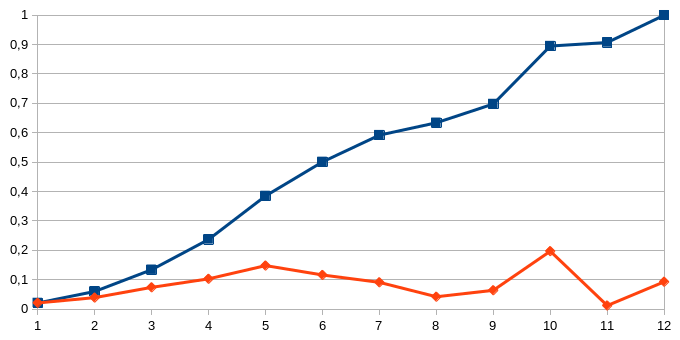
\includegraphics[width=.65\textwidth]{pdf_plots/hashinv_exampleFuncPlot.pdf}
        \caption{Verteilungsfunktion F (orange) und ihre kumulative Dichte $\mathrm{C_F}$}
    \end{figure}
\end{frame}

\begin{frame}{Hash-basierte Inversionsmethode: Beispiel}
    \begin{table}%[htb!]
        \centering
        \begin{tabular}{l|l<{\onslide<2->}|l<{\onslide<5->}|c@{\hspace{\tabcolsep}\onslide<7->\onslide}}
            $X_j$   & $\mathrm{C_F}(X_j)$  & $I_j$ & T$(I_j)$ \\
            \hline\hline % & & & \\
            $v_1$   & $0.021$   & $1$   & $1$ \\ 
            $v_2$   & $0.060$   & $1$   & $1$ \\
            $v_3$\cellcolor<5>{pyorange}   & $0.134$   & $2$\cellcolor<4-5>{pyblue}   & $3$\cellcolor<5>{pyorange} \\
            $v_4$\cellcolor<5>{pyorange}   & $0.237$   & $3$\cellcolor<4-5>{pyblue}   & $4$\cellcolor<5>{pyorange} \\
            $v_5$   & $0.385$   & $4$   & $5$ \\
            $v_6$   & $0.501$   & $6$   & $6$
        \end{tabular}
        \hspace{2em}
        \begin{tabular}{l|l<{\onslide<3->}|l<{\onslide<7->}|c@{\hspace{\tabcolsep}\onslide<5->\onslide}}
            $X_j$   & $\mathrm{C_F}(X_j)$  & $I_j$ & T$(I_j)$ \\
            \hline\hline % & & & \\
            $v_7$   & $0.592$   & $6$   & $6$ \\ 
            $v_8$\cellcolor<7>{pyorange}   & $0.634$   & $7$\cellcolor<6-7>{pyblue}   & $8$\cellcolor<7>{pyorange} \\
            $v_9$   & $0.698$   & $7$\cellcolor<6-7>{pyblue}   & $8$\cellcolor<7>{pyorange} \\
            $v_{10}$& $0.895$   & $9$   & $10$ \\ 
            $v_{11}$& $0.907$   & $10$  & $11$ \\
            $v_{12}$& $1.000$   & $11$  & $12$
        \end{tabular}
        \caption{\small\cite{chen_asau-generating_random_variates-1974}\normalsize}
    \end{table}
\end{frame}

\begin{frame}{Hash-basierte Inversionsmethode: Beispiel}
    \begin{minipage}{.47\textwidth}
        $\textbf{u = 0.642}$
        \begin{itemize}
            \item<2-> $I_u = \lfloor u * 10\rfloor + 1 = 7$
            \item<3-> $i = \mathrm{T}(I_u) = \mathrm{T}(7) = 8$
            \item<4-> $r$ ist nächstgrößerer Index, sodass T$(v_r)\neq \mathrm{T}(v_i)$, also $r = 10$
            \item<5-> F$(v_{i-1}) < u \leq \mathrm{F}(v_r)$
            \item<7-> $u < \mathrm{F}(v_9)\rightarrow X = v_9$\\[\baselineskip]
        \end{itemize}
        \small\cite{chen_asau-generating_random_variates-1974}\normalsize
    \end{minipage}
    \begin{minipage}{.47\textwidth}
        \begin{table}
            \begin{tabular}{l|l|l|c}
                $X_j$   & $\mathrm{C_F}(X_j)$  & $I_j$ & T$(I_j)$ \\
                \hline\hline % & & & \\
                $v_7$   & $0.592$   & $6$   & $6$ \\ 
                $v_8$   & $0.634$\cellcolor<5>{pyblue}   & $7$\cellcolor<2>{pyblue}   & $8$\cellcolor<3->{pyorange} \\
                $v_9$\cellcolor<7->{pyorange}   & $0.698$\cellcolor<6>{pyblue}   & $7$   & $8$ \\
                $v_{10}$& $0.895$   & $9$   & $10$\cellcolor<4->{pyorange}\\ 
                $v_{11}$& $0.907$   & $10$  & $11$\\
                $v_{12}$& $1.000$   & $11$  & $12$
            \end{tabular}
        \end{table}
    \end{minipage}
\end{frame} 